\begin{comment}
  \bibliography{project.bib}
\end{comment}

\chapter{TGA -- Truevision Graphics Adapter}
\label{cha:tga}

\begin{refsection}

  \cite{91:_truev_tga_file_format_specif}

  \section{Introduction}
  \label{sec:introduction}

  The whole purpose of this book, was to give a good understanding of
  how image formats really work. But we couln't just have jumped right
  in, we required knowledge of how color is stored digitally and how
  some compressin algorithms work. Now it's time to put that knowledge
  to good use. \textit{All} the compressin algorithms we just coverede
  are all used in the image formats we are going to explore. And
  furthermore, the digital color storage model is used extensively in
  image formats.

  Now it's time to explore our first image format: TGA \index{TGA}. But why TGA of
  all image format? Because the format is an extremely simple one at
  that, yet it is actually videly used in some areas, including games
  and video processing. It has all the parts common to all image
  formats and it even features a very simple compression algoriothm:
  RLE, which was one of the algoriothms we covered in the last
  chapter.

  Before we dive let me clarify one thing for you: all data that is
  stored in a computer is just a sequence of number. How this sequence
  of numbers is to be parsed is defined by it's \textit{file format}
  \index{file format}. Thus, the rest of this book will
  simply be about how you parse the meaning of the numbers that an
  image file consists of.

  \begin{figure}[h!]
    \centering
    \inputtikz{im_format.tex}

    \caption{IM image format}
    \label{fig:im}
  \end{figure}

  \section{The general image format}
  \label{sec:general-image-format}

  Please observe figure \ref{fig:im}. It demonstrates a picture of a
  pretty flower in an imaginary
  file format called \textit{IM}. It demonstrated the common elements
  of all image formats. Let's go through them one by one:

  \subsection{Image headers}
  \label{sec:image-headers}

  The first few numbers of an image is its image header \index{image
    header}. This gives general information about an image that
  greatly helps the parsing process. It usually includes information
  like width, height, color depth. It often also includes an
  identification string of the image. Let's look at our example
  image. The first two bytes is two ASCII letters IM. These numbers
  are known as magic numbers \index{magic numbers}. You see, at the beginning of every image
  file there a couple bytes called magic numbers that are common to
  all images of that type. In other words, they help you identify the
  type of the image.

  And following the magic number is the width and height of the
  image. In this case it's width first, but the order is usually
  carefully specified by the image file format's respective
  specificatinons.

  \subsection{Color palette}
  \label{sec:color-pallete}

  Color palettes \index{color palette} are also very common, but far
  from all images use them, but as good as image format support them,
  hence why they are included in this sample format. A color palette
  is basically an array or list. And each element of this list is a
  color stored as we talked about in chapter \ref{cha:color}.

  \subsection{The color data}
  \label{sec:color-data}

  Following the header and the optinal color palette is the actual
  color data. If a color palette in indeed used, this section will
  only contain index number to the color palette. Otherwise, it will
  contain a long stream of color, stored in the color-depth specified
  in the header.

  But it's not really that easy. A majority of all image format have
  had some sort of compression applied to their color data. Because it
  just isn't feasible to store them in raw format \index{raw
    format}. Photgraphies for example, contains thousands perhaps even
  tenthousands of very varying color data. \todo{find actual
    statistics for this claim.}. Not even for images with very simple
  and non varying color data like logos \todo{give example}, is this
  method good for. It doesn't do try to find the very similar color
  data and do compression. Even a very,very simple compression like RLE
  algorithm can do wonder on an image such as \todo{make the logo},
  cutting down the size by maybe even thousands of kilobytes!

  \todo{show both an example photography and a logo}

  \begin{figure}[h!]
    \centering
    \newcommand{\shieldcolor}{red}
    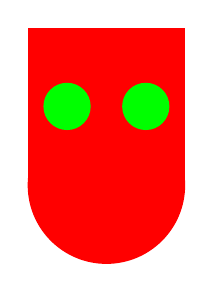
\begin{tikzpicture}
      \fill[\shieldcolor] (0,0) rectangle (2,2);
      \fill[\shieldcolor] (1,0) circle (1);

      \fill[green] (0.5,1) circle (0.3);
      \fill[green] (1.5,1) circle (0.3);
      
    \end{tikzpicture}
    \caption{Fake logo}
    \label{fig:logo}
  \end{figure}

  \printbibliography[heading=subbibliography]

\end{refsection}